
\section{Manipulating deformable objects} \label{sec:lit_traditional}
The goal of this section is to provide important historical context and work in the rigid and deformable object manipulation literature. First, we discuss the traditional approach to rigid object manipulation for robots. This is to show how the vast amount of work in rigid object manipulation is hard to generalize towards deformable object manipulation. Next, we provide a definition and categorization of deformable objects. For each of the categories, we provide common tasks and solutions identified in literature. Finally, we highlight important work in the domain of robotic folding.

\subsection{Manipulating rigid objects}
Grasping and manipulation problems in robotics are traditionally solved by manually engineering subsystems for perception, planning and control~\autocite{Siciliano2008}. A popular approach is to use images as input observation for controlling the motions of the robot. This is motivated by the advantage that images enable closed-loop control: non-contact and real-time measurements of the environment can be used to provide feedback to the motion trajectory of the robot. This principle is generally known as visual servoing~\autocite{Hutchinson1996} and was first introduced in ~\citeyear{Hill1979} by~\textcite{Hill1979}. An archetypical pipeline consists of the following steps to grasp and manipulate an object~\autocite{Corke1996}. First, observations such as images are used to estimate the state of the object. This state estimation stage usually executes pixel manipulations and image filtering in order to extract features. This object state is in turn used for interpreting the scene in order to calculate the relative position of the target object from the robot end-effector. Once the object is identified, it can be modelled such that a suitable grasping point can be identified. Next, these grasping points are given to a motion planning system that calculates a trajectory to move the end-effector to the desired position and orientation. Finally, a low-level controller sends motor commands to the actuators to move the robot.

% TODO: add figure of some typical modular pipeline
\tikzstyle{block} = [rectangle, draw, fill=blue!15, text width=8.0em, minimum height=1cm, text centered, rounded corners]
\begin{figure}[htbp!]
    \centering
    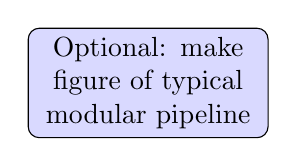
\begin{tikzpicture}[auto, align=center]]
        \node (mock) [block] {Optional: make figure of typical modular pipeline};
    \end{tikzpicture}
    \caption{Optional figure that demonstrates a typical modular pipeline where errors acccumulate.}
\end{figure}

% Probleem met traditionele pipelines toepassen voor vervormbare objecten
Engineering modular, hand-tuned motor control pipelines have been successful for applications in manufacturing~\autocite{Clocksin1985,Mochizuki1987}, car steering~\autocite{Dickmanns1988}, robotic ping-pong~\autocite{Andersson1987}, juggling~\autocite{Rizzi1993} as well as fruit picking~\autocite{Harrell1989}. However, all of these applications operate under the condition of rigid objects: the shape of the object will not change on contact. When manipulating objects, this is of importance for determining stable grasping points. More concretely, restraining rigid objects relies on \textit{form closure}~\autocite{Nguyen1988} or \textit{force closure}~\autocite{Bicchi1995}: fully constraining relative motion of the object or having contact points that can counteract an external wrench through friction. % TODO optional: foto toevoegen: form closure: portefuille volledig vastgrijpen (zie robotics springer bible pagina 1023, fig 38.6 en fig 38.8)
However, in the case of deformable objects, the object can deform during grasping and manipulation. This leads to exponentially higher dimensional configuration spaces~\autocite{Foresti2004} compared to rigid object manipulation. For example, achieving form closure becomes impossible as it requires immobilizing every degree of freedom. Similarly, force closure becomes computationally intractable as it requires constantly incorporating the adapted shape of the object. Furthermore, manipulation requires reasoning about the target shape of the object. These properties make many of the rigid object manipulation techniques hard to extent in the deformable object domain. Unfortunately, to date, the vast majority of robotic manipulation work deals with rigid objects whereas many objects are of deformable nature~\autocite{Siciliano2008}.

\subsection{Deformable objects: definition, categorization, tasks and solutions}
% Vervormbare objecten: wat zijn ze, categorisatie, welke taken en welke oude pipelines bestaan er
A deformable object is an object whose shape changes when being subject to an external force. This deformation can be temporary and reversible (\textit{elastic}), permanent (\textit{plastic}) or a combination of both (\textit{elasto-plastic}). Deformable objects are found both in industrial settings and household items. A common categorization~\autocite{Saadat2002,Jimenez2012} is based on the geometry of the object: how many dimensions are significantly larger than the other dimensions. In its simplest setting, the deformable object is one dimensional: ropes, strings, cables, threads and catheters among others. These objects are also known as deformable linear objects. The term \textit{linear} refers to one dimension being dominant over the other two dimensions. Common tasks for deformable linear objects are grasping, manipulation, sensing and knot tying. Early motor control architectures for solving tasks regarding deformable linear objects used either an open-loop approach or simple visual servoing to execute the motion. An early work demonstrating modular motor control pipelines clearly is the project of~\citeauthor{Inaba1987} in~\citeyear{Inaba1987}. Their method employs visual servoing for manipulating a rope into a ring and then tying the rope. Their perception module uses stereo images to detect the rope and the ring. The planning module is hard-coded to iterate through a set of predefined steps while using the detected center of the ring and 3D coordinates of the endpoints of the rope from the perception module. An inverse kinematics module provides a target trajectory to the low-level controller. Similar modular pipelines can be found in~\autocite{Remde1999} for grasping a rope and in~\autocite{Saha2007} where knots are tied with needles using probabilistic trajectories of the rope from a simulated model. Incorporating motion primitives, i.e. a predefined set of motor actions corresponding to high-level actions, in the planning module is used in~\autocite{Yamakawa2008, Vinh2012} to tie knots in a rope.

% TODO: add figure of some DLO's
\tikzstyle{block} = [rectangle, draw, fill=blue!15, text width=8.0em, minimum height=1cm, text centered, rounded corners]
\begin{figure}[htbp!]
    \centering
    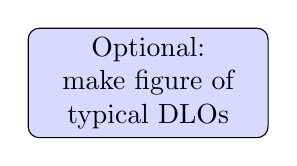
\begin{tikzpicture}[auto, align=center]]
        \node (mock) [block] {Optional: make figure of typical DLOs};
    \end{tikzpicture}
    \caption{Optional figure.}
\end{figure}

% 2D objects klassieke pipelines
Deformable \textit{linear} objects become deformable \textit{planar} objects when two dimensions are significantly larger than the third dimension. In this case, the planning module can disregard the thickness of the material for manipulation. Canonical examples of such objects are clothing, thin-shelled objects like plastic bottles, fabric, paper, paper and plastic bags, deformable sheets, cards and foam materials. A classic example of paper folding is robotic origami in which a robot has to sculpt a piece of paper into a desired shape by folding. This problem was tackled with an open-loop control architecture in~\autocite{Balkcom2008} to produce a folded hat.~\Textcite{Elbrechter2012} take this a step further by using vision, simulation and fiducial markers on the paper to grasp and fold a paper with a five-fingered end-effector. Related to origami is carton folding and metal sheet bending. Typical control strategies~\autocite{Liang1999,Liu2003,Aomura2002} consist of finding the correct locations and sequence of bending operations by modeling the object as a collection of panes articulated through hinge joints. Robotic manipulation of bags has been less studied due to the complexity of modeling and manipulating bags. Dedicated hardware has been researched for grasping~\autocite{Kazerooni2005} and unloading~\autocite{Kirchheim2008} sacks. A general-purpose two-fingered robotic gripper is used in~\autocite{Klingbeil2011} to grasp objects from a table, search the barcode and drop the object into a bag. The planner uses 3D points clouds of depth images taken by a camera. However, they assume the bag is already open for insertion and do not consider any possible deformations caused by touching or dropping an item into the bag.

In context of this thesis, it is of interest to note that garments satisfy the same geometrical property of having one negligible dimension as objects such as paper and plastic bottles. However, the main characteristic distinguishing cloth is the compression strength: compared to other two-dimensional deformable objects, cloth does not possess any significant compression strength. Given that the current work deals with manipulations of clothing items, we focus in particular on cloth manipulation pipelines in Subsection~\ref{subsec:lit_cloth_folding_pipelines}.

% TODO: add figure of some planar deformable objects
\tikzstyle{block} = [rectangle, draw, fill=blue!15, text width=8.0em, minimum height=1cm, text centered, rounded corners]
\begin{figure}[htbp!]
    \centering
    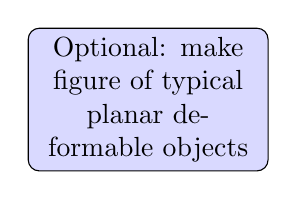
\begin{tikzpicture}[auto, align=center]]
        \node (mock) [block] {Optional: make figure of typical planar deformable objects};
    \end{tikzpicture}
    \caption{Optional figure.}
\end{figure}

% 3D objects klassieke pipelines
The final category of deformable objects are \textit{solid deformable objects} whose deformations across all dimensions of the object are of relevance. These are objects such as food, plush toys and sponges. In general, 3D deformable objects are the least researched type of deformable objects~\autocite{Sanchez2018}. An exception to this is soft tissue which is of importance for medical application. We refer the reader to the review paper by~\textcite{Taylor2016} for an overview of medical robots in surgery applications. For an overview on robotic manipulation of food products, we refer to the survey by~\textcite{Chua2003}.
% TODO: add figure of some 3D deformable objects
\tikzstyle{block} = [rectangle, draw, fill=blue!15, text width=8.0em, minimum height=1cm, text centered, rounded corners]
\begin{figure}[htbp!]
    \centering
    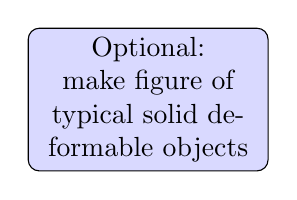
\begin{tikzpicture}[auto, align=center]]
        \node (mock) [block] {Optional: make figure of typical solid deformable objects};
    \end{tikzpicture}
    \caption{Optional figure.}
\end{figure}

\subsection{Cloth manipulation pipelines} \label{subsec:lit_cloth_folding_pipelines}
%  wat is het doel van deze subsectie?  = Inzicht verschaffen in hoe "klassieke" pipelines het probleem opdelen (is al geschreven :)) en hoe ze die problemen typisch aanpakken. Doel is dat lezer hieruit kan afleiden dat dat wel cool is maar: traag, error accumulation, geen knowledge reuse etc. 
% Cloth folding pipelines (houvast = Sanchez2018, Matas, Douman2016)
It is possible to distinguish multiple task when considering cloth manipulation applications: sensing, grasping, manipulation and cloth-specific tasks such as folding, cloth hanging and bedsheet folding. A complete cloth folding pipeline typically consists of the following subtasks: (1) grasping an isolated garment, (2) bringing it into a folded configuration and (3) stacking it on top of other folded garments. The second step in this process is often subdivided into unfolding, flattening and folding. Most of the work in robotic folding deal with a subtask instead of the complete pipeline. A notable exception is the work of~\textcite{Doumanoglou2016,Maitin2010} that consider the whole robotic folding pipeline.
% TODO: add figure of robotic folding pipeline
\tikzstyle{block} = [rectangle, draw, fill=blue!15, text width=8.0em, minimum height=1cm, text centered, rounded corners]
\begin{figure}[htbp!]
    \centering
    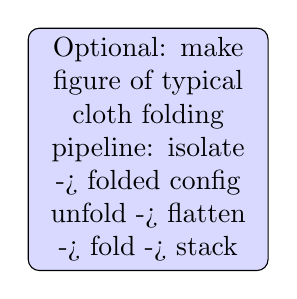
\begin{tikzpicture}[auto, align=center]]
        \node (mock) [block] {Optional: make figure of typical cloth folding pipeline: isolate -> folded config {unfold -> flatten -> fold} -> stack};
    \end{tikzpicture}
    \caption{Optional figure.}
\end{figure}

An evident solution for cloth folding is to use specialized hardware in a constrained environment.~\Textcite{Nair2013} propose an actuated flipfold\footnote{A flipfold is a device consisting of four panels joined by hinges. The four panels lineup with the two sleeves, top-center and bottom-center of the shirt respectively. The hinges allow the panels to rotate inwards. This movement takes the cloth with it and as such makes the folds.} that automates folding of shirts. More complex commercially available products exists such as the FoldiMate\footnote{\url{https://foldimate.com/}}. However, such products do not generalize towards general cloth folding, do not leverage general-purpose robotic hardware and have proven difficult to bring commercially available\footnote{FoldiMate has been in prototype development for nine years at time of writing.}. This is why most research consider the use of general-purpose robot arms, possibly with dedicated gripper and instrumentation, as elaborated in Section~\ref{sec:lit_instrumentation}.

Much of the literature around cloth folding has resolved around solving subtasks of the folding pipeline. In the following paragraphs, we provide a summary of important work concerning each of the subtasks and describe two important works that consider the complete folding pipeline.

\paragraph{Grasping.}
Grasping a piece of cloth requires isolating a single piece of garment from a pile of clothing articles and making sure that one functional piece is grasped. In~\autocite{Ramisa2012}, this is done by grasping shirts via the collar. Visual servoing is used with preprocessed features on depth data. Their method achieves a grasping success rate of $70\%$. However, the performance drops to $30\%$ when other types of garments are present on the table. ~\autocite{Monso2012} separate all clothing articles with a robot manipulator. Occlusion of clothing articles leads to uncertainty of the state estimation. They model this explicitly by training a \acrshort{POMDP} for the cloth state estimation.

\paragraph{Pose estimation.}
After grasping a clothing article, pose estimation is usually done such that the type and configuration of the cloth can be brought into an unfolded state, ready for folding. Garment pose estimation has been done by matching video images to simulation models~\autocite{Kita2002}, using machine learning models~\autocite{Li2014, li2014volum} or instrumentation via fiducial markers~\autocite{Bersch2011}.

\paragraph{Unfolding.}
Unfolding is an important step as it allows to bring the article into a known configuration from which predefined folding strategies can be employed. A general approach to unfold clothing articles is to exploit gravity; by grasping the article at strategic points, gravity will remove arbitrary folds. ~\Textcite{Hamajima1998} exploit this gravitational trick by regrasping the hemlines of the garments. The hemlines are detected using the shadows and shape of the cloth. \textcite{Cusumano2011} unfolds shirts and trousers in a two-staged pipeline using \acrshortpl{HMM}, a cloth simulator and a planning algorithm. By inputting the clothing article type, size and grasping points for the gripper to the \acrshort{HMM}, it can estimate the garment's configuration. This configuration is used by the simulation model to find the minimum-energy configuration. This is the configuration in which the garments triangulated mesh vertices have minimum gravitational potential energy. Then, the planning module repeatedly executes trajectories to regrasp the clothing article until it is in a known configuration. Then, the planning module brings the garment into the hard-coded, unfolded configuration. Their method achieves a $66\%$ success rate. \textcite{Doumanoglou2014} solves the same task but reduces the amount of software modules by repeatedly regrasping the lowest hanging point of the garment. This brings the clothing item into a known configuration. Next, the robot unfolds the article by searching two grasping points using a \acrshort{POMDP}.

\paragraph{Flattening.}
Before folding the cloth into the desired configuration, it is necessary to remove wrinkles caused by unfolding the cloth. Moreover, folding often relies on template matching which is made more difficult when there are wrinkles present. A dedicated method for cloth flattening is proposed in~\autocite{Sun2015}. Their method assumes the clothing item is unfolded on a table. They employ RGB-D data to find wrinkles and represent them as fifth-order polynomials. The largest wrinkle is then flattened by using preprogrammed motions of the arms. In ~\autocite{Willimon2011}, a washcloth is flattened in two phases. In the first phase, they iteratively pull the cloth away from or towards its centroid to remove minor wrinkles. The second phase utilizes depth information to determine regions of interests with high degree of wrinkles and the necessary direction for removing them.

\paragraph{Folding.}
\Textcite{Bersch2011} execute an open-loop motor control trajectory to fold clothing after unfolding it using fiducial markers on the cloth. The folding loop exhibits a common human strategy to fold cloth: grasp the garment by the shoulders, rotate the sleeves inwards and fold the shirt inwards while placing it on the table. In~\autocite{Berg2010}, they employ a geometry based folding method which folds over predefined lines. Their method relies on using gravity to immobilize parts of the garment such that parts of the cloth become rigid objects.~\autocite{Miller2012} estimate the pose of the garment by fitting a user-specified polygon representation to the detected cloth contours. Then, they apply the same method as~\autocite{Berg2010} to fold the cloth. \Autocite{Yamakawa2011} start folding a cloth in midair, held by its corners, with an algebraic representation of the cloth. They use this simulation model to estimate the pose of the end-effectors at exact intervals such that open-loop trajectory of the points describes a folded garment. Contrary to previous mentioned approaches which rely on a dual-robot arm platform,~\autocite{Petrik2017} considers folding with a single robotic arm. They compute a trajectory in simulation based on the grasping location and the folding line of the garment. However, the literature concerning folding with a single robotic arm is rather scarce due to its limited applications.

\paragraph{Full pipeline.}
The first example of a complete cloth folding pipeline is the work of~\textcite{Maitin2010}. The task starts from an unorganized pile of crumbled towels and ends when all articles are stacked in folded configuration on top of each other. Given that the end of their pipeline consists of executing predefined trajectories, much of their method rely on predecessor steps to bring the clothing into an exactly known configuration. Their method start with color segmentation on the image to select the central clothing article. Next, the grasped towel is rotated and regrasped in order to find and grasp the corners visually. Unfolding is done by shaking and twisting, and pulling the towel taut. Finally, they run a predefined, open-loop trajectory to lay down the unfolded towel on the table and fold it. The pipeline takes $24$ minutes to execute with the grasp point detection phase being the largest bottleneck.

The second full robotic cloth folding implementation is engineered by~\citeauthor{Doumanoglou2016}. Their setup considers folding  a pile of shirts, towels and trousers. By segmenting an image from the pile on color, an isolated piece is grasped. By repeatedly regrasping the lowest hanging point of the garment, they reduce the amount of possible cloth configuration to classify the garment shape using random forests~\autocite{Breiman2001}. The unfolding procedure is equivalent to~\autocite{Maitin2010} and requires a garment classifier, grasp point detector, and a pose estimation module. Flattening the shirt is done using a brush tool on a dedicated cloth folding gripper. Wrinkles are detected by comparing the contours with existing polygonal models of flattened cloths. Finally, the fold is executed by polygon matching of the contours to predefined templates. Their system achieves a throughput of six minutes per garment with $79\%$ success rate. The slowest step in their pipeline is the detection of the desired grasping points for unfolding.

As concluding remark of this section, we observe a reoccurring theme: a divide-and-conquer methodology leads to a loss of information between the different stages, resulting in the accumulation of errors. For example,~\textcite{Doumanoglou2016} report difficulties when folding towels because the perception system labels them as shirts. These individual components are built in a laboratory environment with certain assumptions which are likely to be violated in an unstructured, complex environment. Inaccurate sensor readings together with deformation of the robot’s links also deteriorate the accuracy of these systems. In order for robots to be useful in unstructured environments with complex dynamics, there is a need for controllers that are able to perform robust grasp synthesis when faced with unseen conditions.